
% ===============================================
% MATH 34: Multivariable calculus           Spring 2019
% hw_template.tex
% ===============================================

% -------------------------------------------------------------------------
% You can ignore this preamble. Go on
% down to the section that says "START HERE" 
% -------------------------------------------------------------------------

\documentclass{article}

\usepackage[margin=1.5in]{geometry} % Please keep the margins at 1.5 so that there is space for grader comments.
\usepackage{amsmath,amsthm,amssymb,hyperref}
\usepackage{graphicx}
\usepackage{float}
\usepackage{listings}
\usepackage{xparse}
\usepackage{xcolor}
\usepackage{verbatim}

\newcommand{\R}{\mathbf{R}}  
\newcommand{\Z}{\mathbf{Z}}
\newcommand{\N}{\mathbf{N}}
\newcommand{\Q}{\mathbf{Q}}
\newcommand{\C}{\mathbf{C}}
\newcommand{\Log}{\text{Log}}
\newcommand{\Arg}{\text{Arg}}
\newcommand{\Real}{\text{Re}}
\newcommand{\Imag}{\text{Im}}
\newcommand{\ddz}{\frac{d}{dz}}

\newenvironment{theorem}[2][Theorem]{\begin{trivlist}
\item[\hskip \labelsep {\bfseries #1}\hskip \labelsep {\bfseries #2.}]}{\end{trivlist}}
\newenvironment{lemma}[2][Lemma]{\begin{trivlist}
\item[\hskip \labelsep {\bfseries #1}\hskip \labelsep {\bfseries #2.}]}{\end{trivlist}}
\newenvironment{claim}[2][Claim]{\begin{trivlist}
\item[\hskip \labelsep {\bfseries #1}\hskip \labelsep {\bfseries #2.}]}{\end{trivlist}}
\newenvironment{problem}[2][Problem]{\begin{trivlist}
\item[\hskip \labelsep {\bfseries #1}\hskip \labelsep {\bfseries #2.}]}{\end{trivlist}}
\newenvironment{proposition}[2][Proposition]{\begin{trivlist}
\item[\hskip \labelsep {\bfseries #1}\hskip \labelsep {\bfseries #2.}]}{\end{trivlist}}
\newenvironment{corollary}[2][Corollary]{\begin{trivlist}
\item[\hskip \labelsep {\bfseries #1}\hskip \labelsep {\bfseries #2.}]}{\end{trivlist}}

\newenvironment{solution}{\begin{proof}[Solution]}{\end{proof}}

\makeatletter
\newcommand{\skipitems}[1]{%
	\addtocounter{\@enumctr}{#1}%
}
\makeatother

\NewDocumentCommand{\codeword}{v}{%
\texttt{\textcolor{blue}{#1}}%
}


\begin{document}

\large % please keep the text at this size for ease of reading.

% ------------------------------------------ %
%                 START HERE             %
% ------------------------------------------ %

{\Large Page 1 % Replace with appropriate page number 
\hfill  MTH483, Complex Variables, HW5}

\begin{center}
{\Large Wyatt Whiting}
\end{center}
\vspace{0.05in}

% -----------------------------------------------------
% The "enumerate" environment allows for automatic problem numbering.
% To make the number for the next problem, type " \item ". 
% To make sub-problems such as (a), (b), etc., use an "enumerate" within an "enumerate."
% -----------------------------------------------------
\begin{enumerate}
	\item Problem 4.18, page 70
	
	$\gamma := (4+0i)+t(-4+4i)=4-4t+4it, t\in [0,1]$
		
	$\gamma '=-4+4i$
	\begin{enumerate}
		\item
		\[\int_{\gamma}\frac{z+1}{z}dz=[\Log(z)+z]_{4}^{4i}=(\Log(4i)+4i)-(\Log(4)+4) \]
		\[(\ln|4i|+i\Arg(4i)+4i)-(\ln|4|+i\Arg(4)+4)=4+i\left(\frac{\pi}{2}+4\right) \]
		
		\item
		\[\int_{\gamma}\frac{dz}{z^2+z}=[\Log(z)-\Log(z+1)]_{4}^{4i} = \]
		\[=[\Log(4i)-\Log(1+4i)]-[\Log(4)-\Log(5)] \]
		\[=[\ln|4i|+i\Arg(4i)-\ln|1+4i|-i\Arg(1+4i)] - [\ln|4|+i\Arg(4)-\ln|5|-i\Arg(5)] \]
		\[=i\Arg(4i)-\ln(\sqrt{17})-i\Arg(1+4i)+\ln(5) \]
		\[=\ln\left(\frac{5}{\sqrt{17}}\right)+i\left(\frac{\pi}{2}-\arctan(4)) \right) \]
		
		\item 
		\[\int_{\gamma}z^{-\frac{1}{2}}dz=\left[2z^{\frac{1}{2}} \right]_{4}^{4i} \]
		\[=\left[ 2(4i)^{\frac{1}{2}}   \right]-\left[ 2(4)^{\frac{1}{2}}  \right] \]
		\[ =2(e^{\frac{1}{2}\ln4+\frac{1}{2}i\frac{\pi}{2}})- 4 \]
		\[=2(2e^{i\frac{\pi}{4}} )-4\]
		\[=4e^{i\frac{\pi}{4}}-4=4(e^{i\frac{\pi}{4}}-1) \]
		
		\item 
		\[\int_{\gamma}\sin^2(z)dz=\left[ \frac{z}{2}-\frac{\sin(z)\cos(z)}{2}  \right]_{4}^{4i} \]
		\[=\left[ \frac{4i}{2}-\frac{\sin(4i)\cos(4i)}{2}  \right] -\left[ \frac{4}{2}-\frac{\sin(4)\cos(4)}{2}  \right]\]
		\[=2i-i\frac{\sinh(4)\cosh(4)}{2}-2+\frac{\sin(4)\cos(4)}{2} \]
		\[=\frac{\sin(4)\cos(4)}{2}-2+i\left(2-\frac{\sinh(4)\cosh(4)}{2}\right) \]
	\end{enumerate}
	
	\item Problem 4.19, page 70
	\begin{enumerate}
		\item $\gamma_1(t)=e^{it}, -\frac{\pi}{2}\leq t \leq \frac{\pi}{2}$
		
		$\gamma_1 '(t)=ie^{it}$
		\[\int_{\gamma_1}z^i dz = \int_{\gamma_1}e^{i\Log(z)}dz \]
		\[=\int_{-\pi/2}^{\pi/2}e^{i(\ln|e^{it}|+i\Arg(e^{it}))}ie^{it}dt= \int_{-\pi/2}^{\pi/2}e^{i(it)}ie^{it}dt\]
		\[=\int_{-\pi/2}^{\pi/2}ie^{it-t}dt=\left[\frac{e^{it-t}}{2}-\frac{ie^{it-t}}{2} \right]_{-\pi/2}^{\pi/2} \]
		\[=\frac{e^{i\frac{\pi}{2}-\frac{\pi}{2}}}{2} - \frac{ie^{i\frac{\pi}{2}-\frac{\pi}{2}}}{2} - \frac{e^{-i\frac{\pi}{2}+\frac{\pi}{2}}}{2} + \frac{ie^{-i\frac{\pi}{2}+\frac{\pi}{2}}}{2} \]
		\[=\frac{ie^{-\pi/2}}{2} + \frac{e^{-\pi/2}}{2} + \frac{ie^{\pi/2}}{2} + \frac{e^{\pi/2}}{2} \]
		\[=\frac{e^{-\pi/2}+e^{\pi/2}}{2}  + i\frac{e^{-\pi/2}+e^{\pi/2}}{2}\]
		
		
		\item $\gamma_2(t)=e^{it}, \frac{\pi}{2}\leq t \leq \frac{3\pi}{2}$
		
		For this problem, we must redefine the $\Log$ function since taking the principle logarithm over the given interval would prove unfruitful. I will denote the new branch of the logarithm with $\Log^*(z)=\ln|z|+\Arg^*(z)$ where $\Arg^*(z) \in [0, 2\pi )$. Then in a fashion like the previous part,
		
		\[\int_{\gamma_2}z^i dz = \int_{\gamma_2}e^{i\Log^*(z)}dz \]
		\[=\int_{\pi/2}^{3\pi/2}e^{i(\ln|e^{it}|+i\Arg^*(e^{it}))}ie^{it}dt= \int_{\pi/2}^{3\pi/2}e^{i(it)}ie^{it}dt\]
		\[=\int_{\pi/2}^{3\pi/2}ie^{it-t}dt=\left[\frac{e^{it-t}}{2}-\frac{ie^{it-t}}{2} \right]_{\pi/2}^{3\pi/2} \]
		\[= \frac{e^{i\frac{3\pi}{2}-\frac{3\pi}{2}}}{2} - \frac{ie^{i\frac{3\pi}{2}-\frac{3\pi}{2}}}{2} - \frac{e^{i\frac{\pi}{2}-\frac{\pi}{2}}}{2} + \frac{ie^{i\frac{3\pi}{2}-\frac{3\pi}{2}}}{2}  \]
		\[=-\frac{ie^{\frac{-3\pi}{2}}}{2} - \frac{e^{\frac{-3\pi}{2}}}{2} - \frac{ie^{\frac{-\pi}{2}}}{2}-\frac{e^{\frac{-\pi}{2}}}{2} \]
		\[=\frac{-e^{\frac{-3\pi}{2}}-e^{\frac{-\pi}{2}}}{2} + i\frac{-e^{\frac{-3\pi}{2}}-e^{\frac{-\pi}{2}}}{2} \]
	\end{enumerate}
	
	\item Evaluate the following integrals where the circle is positively oriented,
	\begin{enumerate}
		\item This function does not have an antiderivative along the specified path, so we will apply Cauchy's Integral Formula. Let $\gamma := C_2(-1)$ with positive orientation.
		
		\[\int_{\gamma}\frac{z^2}{4-z^2}dz=\int_{\gamma}\frac{1}{z+2}-\frac{1}{z-2}-1dz = \int_{\gamma}\frac{1}{z+2}dz - \int_{\gamma}\frac{1}{z-2}dz-\int_{\gamma}dz \]
		
		By Cauchy's Integral formula we have
		
		\[\int_{\gamma}\frac{1}{z+2}dz=2\pi i \]
		
		It should also be clear that by the Cauchy-Goursat theorem,
		
		\[\int_{\gamma}1dz = 0.\]
		
		Since we know that 
		
		\[\int_{\gamma}\frac{1}{z-2}dz=\log(z-2)+c \]
		where $\log$ has some branch cut, we can choose any branch cut that doesn't not intersect $\gamma$ which is possible since the "center" of the cut lies outside the circle. Then $\frac{1}{z-2}$ is holomorphic and continuous on $G=\gamma \cup \partial\gamma$, so by Cauchy-Goursat we have
		
		\[\int_{\gamma}\frac{1}{z-2}dz= 0. \]	
		So then we have 
		
		\[\int_{\gamma}\frac{z^2}{4-z^2}dz=2\pi i \]
		\item We know $C_1(0)$ is a simple loop with positive orientation. $\sin(z)$ is holomorphic on $\C$ and 0 is contained within $C_1(0)$. Thus we can apply Cauchy's Integral formula, giving
		
		\[\int_{\gamma}\frac{\sin(z)}{z-0}dz=2\pi i\sin(0)=2\pi i(0)=0. \]
	\end{enumerate}
	
	\item $\partial_{xx}u+\partial_{yy}u=0\implies u$ is harmonic.
	\begin{enumerate}
		\item Let $f$ be holomorphic and $f$ is expressible as $f(z)=u(z)+iv(z)$. We then know
		\[\partial_x u = \partial_y v \implies \partial_{xx}u=\partial_{yx}v \]
		and
		\[\partial_y u = -\partial_x v \implies \partial_{yy}u=-\partial_{xy}v. \]
		
		We also know that $\partial_{yx}v=\partial_{xy}v$, so
		\[\partial_{xx}u=\partial_{yx}v=-\partial_{yy}u\implies \partial_{xx}u=-\partial_{yy}u\implies \partial_{xx}u+\partial_{yy}u=0, \]
		so $u$ is harmonic. Likewise we also have
		\[\partial_{xy}u=\partial_{yy}v \]
		\[\partial_{yx}u=-\partial_{xx}v, \]
		so
		\[\partial_{yy}v=\partial_{xy}u=\partial_{yx}u=-\partial_{xx}v \]
		\[ \implies \partial_{yy}v=-\partial_{xx}v \implies \partial_{xx}v+\partial_{yy}v=0, \]
		so $v$ is harmonic as well.
		
		\item Consider the function $g(z)=x=\Real(z)$. Suppose there exits some function $f(z)$ such that $f'(z)=g(z)=x$. Since $f'(z)=(u(z)+iv(z))'=\partial_xu+i\partial_xv$, then it must be the case that $\partial_xu(z)=x\implies u(z)=\frac{x^2}{2}+c$ and $\partial_xv(z)=0\implies v(z)=x+c$. However then we have $\partial_{xx}u=1$ and $\partial_{yy}u=0$, so $\partial_{xx}u-\partial_{yy}u=1\neq 0$, which contradicts the proof from (a). Thus, there is no function $f(z)$ such that $f'(z)=g(z)$, so $g$  has no antiderivatives on $\C$.
	\end{enumerate}
	
	\item Consider the function $f(z)=\frac{1}{z}$.
	\begin{enumerate}
		\item Sketch the horizontal line $y=1/2$ together with its image under f.
		
		\codeword{  ParametricPlot[{ReIm[t + 0.5 I], ReIm[1/(t + 0.5 I)]}, {t, -10, 10}, AxesOrigin -> {0, 0}, PlotRange -> {{-5, 5}, {-2.5, 1}}]   }
		
		This code plots both the line $y=1/2$ and $f(y=1/2)$, with some extra commands to make the graph how I like it.
		\begin{figure}[H]
		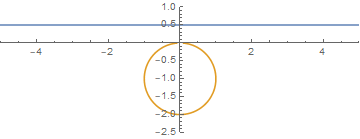
\includegraphics[scale=0.8]{image1.png}
		\end{figure}
		It is interesting to note that an everywhere-positive line becomes everywhere-negative after passing through $f(z)$ as this is not the way inverses would work on the real line. We should also note that the circle does not fully reach the origin. As you trace the horizontal line farther towards positive or negative infinity, the image approaches 0 asymptotically. 
		
		\item Verify that the image of line $y = b > 0$ is a circle. What are its center and radius?
		
		Below I show that various horizontal lines become circles:
		
		\codeword{ParametricPlot[{ReIm[t + 0.25 I], ReIm[1/(t + 0.25 I)]}, {t, -10, 10}, AxesOrigin -> {0, 0}, PlotRange -> {{-5, 5}, {-4, 1}}]}
		
		Same code as before but with modified line height and graphing range
		\begin{figure}[H]
		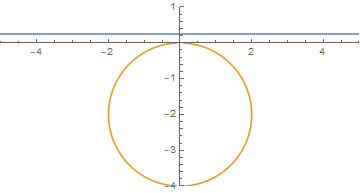
\includegraphics[scale=0.8]{image2.png}
		\end{figure}
		This shows that halving the value of $y$ from 1/2 to 1/4 causes the radius of the circle to double from 1 to 2.
		
		\codeword{ParametricPlot[{ReIm[t + 0 + I], ReIm[1/(t + I)]}, {t, -10, 10}, AxesOrigin -> {0, 0}, PlotRange -> {{-5, 5}, {-1.5, 1.5}}]}
		
		Same code, modified once again.
		\begin{figure}[H]
		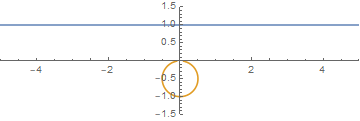
\includegraphics[scale=0.8]{image3.png}
		\end{figure}
		Doubling the height of the line from its initial value halves the radius. The picture now becomes clear.
		
		Given a line $y=b>0$, the image of that line will be a circle with radius $\frac{1}{2b}$ centered at $0-i\frac{1}{2b}$.
		
		\item The image of the half plane is the lower half of the complex plane without the open disc with radius 1 centered at -i.
	\end{enumerate}
	
	\item Consider the function $f(z)=z^3$
	
	\codeword{ParametricPlot[ReIm[(1 + I t)^3], {t, -3, 3}]}
	
	This plots the real and imaginary component of the function along the specified line taking values of $y$ from -3 to 3. It generates the following graph:
	
	\begin{figure}[H]
	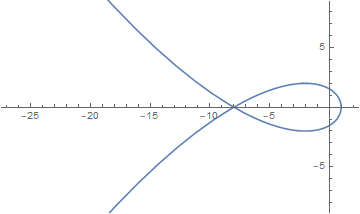
\includegraphics[scale=0.8]{image4.png}
	\end{figure}
	
	\item Take $z_1=1+i\sqrt{3}$ and $z_2=1-i\sqrt{3}$. Then
	
	\[f(z_1)=(1+i\sqrt{3})^3=-8-(1-i\sqrt{3})^3=f(z_2) \]
	
	\item $f(z)=z^3 \implies f'(z)=3z^2$
	
	\[f'(1+i\sqrt{3})=3(1+i\sqrt{3})^2=-6+i6\sqrt{3} \]
	\[f'(1-i\sqrt{3})=3(1-i\sqrt{3})^2=-6-i6\sqrt{3} \]
	
	\item Find the angle at which the path intersects itself. 
	
	The angle at which the image intersects itself is $\frac{2\pi}{3}$.
\end{enumerate}

% ---------------------------------------------------
% Anything after the \end{document} will be ignored by the typesetting.
% ----------------------------------------------------

\end{document}

